%!TEX root = /Users/louis/Documents/PhD/Deliverables/Thesis/thesis.tex

\section{Epsilon HUTN: A Textual Modelling Notation}
\label{sec:notation}
The analysis of co-evolution examples in Chapter~\ref{Analysis} highlighted two ways in which co-evolution is managed. In \emph{developer-driven} co-evolution, migration is specified by the metamodel developer in an executable format; while in \emph{user-driven co-evolution} migration is specified by the metamodel developer in prose or not at all. Performing user-driven co-evolution with modelling frameworks presents two key challenges that have not been explored by existing research. Firstly, user-driven co-evolution often involves editing the storage representation of the model, such as XMI. Model storage representations are typically not optimised for human use and hence user-driven co-evolution can be error-prone. Secondly, non-conformant model elements must be identified during user-driven co-evolution. When a multi-pass parser is used to load models, as is the case with EMF, not all conformance problems are reported at once, and user-driven co-evolution is an iterative process. In Section~\ref{sec:requirements_identification}, these challenges led to the identification of the following requirement: \emph{This thesis must demonstrate a user-driven co-evolution process that enables the editing of non-conformant models without directly manipulating the underlying storage representation and provides a sound and complete conformance report for the original model and evolved metamodel.}

Section~\ref{subsec:migration_with_xmi} illustrates some of the challenges to performing model migration with XMI, and Section~\ref{subsec:alternatives_to_xmi} discusses potential alternatives to XMI for user-driven co-evolution. Section~\ref{subsec:hutn} describes an OMG standard modelling notation that is optimised for human-usability, and Section~\ref{subsec:epsilon_hutn} presents a reference implementation of the OMG standard built atop EMF. Finally, Section~\ref{subsec:migration_with_hutn} demonstrates the wƒay in which the reference implementation of the notation has been integrated with the metamodel independent syntax described in Section~\ref{sec:mmi_syntax} to produce conformance reports. 

\subsection{Model Migration with XMI}
\label{subsec:migration_with_xmi}
The co-evolution example from Section~\ref{sec:mmi_syntax} is now used to illustrate the way in which model migration is performed by editing the underlying storage representation of a model, such as XMI (Section~\ref{subsec:mof}). Consider again the evolution of the families metamodel (Figure~\ref{fig:families_mms_repeated}) and a model conforming to the original metamodel (Figure~\ref{fig:families_model_repeated}).

\begin{figure}[htbp]
	\centering
	\subfigure[Original metamodel.]
	{
	    \label{fig:original_families_mm_repeated}
	    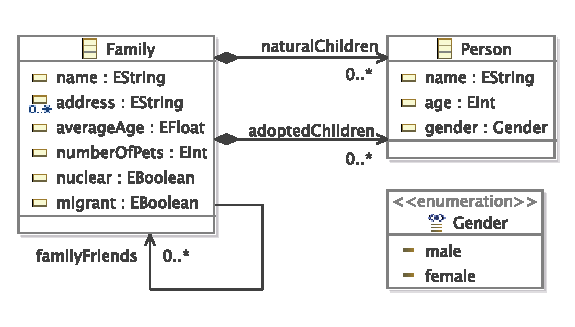
\includegraphics[scale=0.9]{5.Implementation/images/families.pdf}
	}
	\subfigure[Evolved metamodel.]
	{
	    \label{fig:evolved_families_mm_repeated}
	    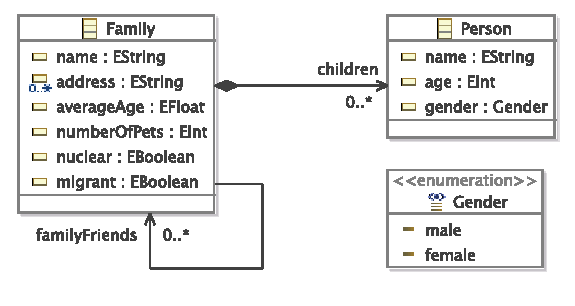
\includegraphics[scale=0.9]{5.Implementation/images/families_evolved.pdf}
	}
	\caption{Evolution of a families metamodel, based on the metamodel in \cite{hutn}.}
\label{fig:families_mms_repeated}
\end{figure}

\begin{figure}[htbp]
  \begin{center}
    \leavevmode
    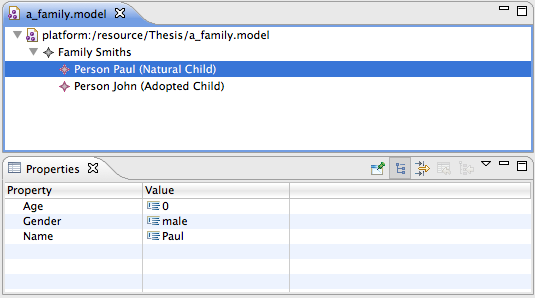
\includegraphics[width=10cm]{5.Implementation/images/family_model.png}
  \end{center}
  \caption[A family model]{A family model, which conforms to the metamodel in Figure~\ref{fig:original_families_mm_repeated}}
  \label{fig:families_model_repeated}
\end{figure}

The model in Figure~\ref{fig:families_model_repeated} does not conform to the evolved metamodel (because it uses the \texttt{na\-tu\-ralCh\-il\-dr\-en} and \texttt{ad\-op\-t\-edCh\-il\-dr\-en} features, which are not defined for \texttt{Pe\-rs\-on}), and hence cannot be loaded by the modelling framework. Migration might be achieved by editing the underlying storage representation directly (i.e. manually manipulating XMI). Listing~\ref{lst:xmi} shows the XMI for the model in Figure~\ref{fig:families_model_repeated}.

\begin{lstlisting}[caption=XMI for the family model in Figure~\ref{fig:families_model_repeated}, label=lst:xmi, language=XML]
<?xml version="1.0" encoding="ASCII"?>
<families:Family xmi:version="2.0" xmlns:xmi="http://www.omg.org/XMI" xmlns:families="families" xmi:id="_kE2LkAagEeC-FIOYrvUj0A" name="Smiths">
  <naturalChildren xmi:id="_q8RWYAagEeC-FIOYrvUj0A" name="Paul"/>
  <adoptedChildren xmi:id="_nj6TcAagEeC-FIOYrvUj0A" name="John"/>
</families:Family>
\end{lstlisting}

XMI is a concrete syntax for models, which has been optimised for use by machines and not by humans \cite{hutn}. Models often contain information that is not relevant to the domain, such as the universally unique identifiers (\texttt{xmi:id} attributes) on lines 2, 3 and 4 of Listing~\ref{lst:xmi}. Furthermore, information is often omitted to reduce the size of the model on disk. For example, the model elements on lines 3 and 4 of Listing~\ref{lst:xmi} do not specify their type (\texttt{Pe\-rs\-on}) and this is inferred from the type of the \texttt{na\-tu\-ralCh\-il\-dr\-en} and \texttt{ad\-op\-t\-edCh\-il\-dr\-en} features. Types are inferred from the metamodel by the modelling framework using a reference from the model to the metamodel. In XMI, metamodel references are expressed using XML namespaces. The XMI in Listing~\ref{lst:xmi} imports the families metamodel to a namespace (families) on line 2. The evaluation presented in Section~\ref{sec:exemplar_user-driven_co-evo} further explores the suitability of XMI for user-driven co-evolution. The remainder of this section discusses the design and implementation of a modelling notation that provides an alternative to XMI, and is tailored for human-use.

\subsection{Potential Alternatives to XMI}
\label{subsec:alternatives_to_xmi}
Two characteristics were considered when designing a notation that provides an alternative to representing models with XMI. Models can be represented textually or graphically (Section~\ref{subsec:modelling_languages}), and with a metamodel-specific or a metamodel-independent syntax (Section~\ref{sec:mmi_syntax}). The benefits and drawbacks of each option have been considered particularly with respect to their implications for user-driven co-evolution, and are now discussed.

\paragraph{Metamodel-independent vs metamodel-specific} A metamodel-specific syntax is defined in terms from the metamodel, and is often more concise than a metamodel-independent syntax. A metamodel-specific (and textual) syntax for part of the original families metamodel (Figure~\ref{fig:original_families_mm_repeated}) is shown in Listing~\ref{lst:mms_syntax}. Using the metamodel-specific syntax, the families model in Listing~\ref{lst:xmi} is represented as \texttt{Smiths:Paul(John)}. Notice that the syntax is defined in metamodel terms, such as \texttt{Fa\-mi\-ly}, \texttt{na\-tu\-ralCh\-il\-dr\-en}, and \texttt{ad\-op\-tedCh\-il\-dr\-en}. Consequently, the syntax definition can be affected by metamodel evolution, and hence cannot be used to load a model that does not conform to the metamodel. Therefore, a metamodel-specific representation is not suitable for use during user-driven co-evolution, which involves using a modelling notation with non-conformant models, and hence a metamodel-independent representation was preferred.

\begin{lstlisting}[caption=A metamodel-specific syntax for families in EBNF, label=lst:mms_syntax, language=EBNF]
family = name ":" naturalChildren "(" adoptedChildren ")"
naturalChildren = name { "," name }
adoptedChildren = name { "," name }
name = "A" | ... | "z"
\end{lstlisting}

\paragraph{Textual vs graphical} For user-driven co-evolution, the usability of the modelling notation is important because a metamodel user manipulates models with the notation to perform migration. The choice between a textual or graphical notation likely has a significant impact on usability, but it was not feasible to conduct a thorough user analysis given the time constraints of the thesis. Instead, a textual notation was selected to reduce implementation effort, and implemented to facilitate the addition of an equivalent graphical notation in future work. In particular, the concrete and abstract syntax definitions of the notation were kept separate to simplify the addition of an alternative concrete syntax in the future.

Currently, several tools exist for representing models with textual and metamodel-specific syntaxes (such as the text-to-model transformation tools discussed in Section~\ref{subsubsec:model_transformation}), but no tools exist for representing models in a metamodel-independent syntax other than XMI. \cite{steel01hutn} describe the Distributed Systems Technology Centre's TokTok project, which provided a metamodel-independent textual modelling notation, and is now inactive. \cite{muller05hutn} describe a me\-ta\-mo\-del-inde\-pe\-nd\-ent representation, which they have since abandoned in favour of Sintaks\footnote{\url{http://www.kermeta.org/sintaks/}}, a tool for constructing metamodel-specific representations.

\cite{steel01hutn,muller05hutn} based their me\-ta\-mo\-del-independent representations on an OMG standard, Human-Usable Textual Notation (HUTN), which defines a textual modelling notation that aims to conform to human-usability criteria \cite{hutn}. As a me\-ta\-mo\-del-inde\-pe\-nd\-ent and textual concrete syntax, HUTN was seen as an ideal starting point for designing a textual modelling notation for user-driven co-evolution. OMG HUTN is described in the sequel.

\subsection{OMG Human-Usable Textual Notation}
\label{subsec:hutn}
OMG HUTN is a textual, metamodel-independent modelling notation whose primary design goal is human-usability and ``this is achieved through consideration of the successes and failures of common programming languages'' \cite[Section 2.2]{hutn}. The HUTN specification refers to two studies of programming language usability to justify design decisions. However, the OMG specification does not evaluate the human-usability of the notation because no reference implementation exists. As HUTN is (purportedly) optimised for human-usability, using HUTN rather than XMI for user-driven co-evolution should lead to increased developer productivity. This claim is explored in Chapter~\ref{Evaluation}.

Like the metamodel presented in Section~\ref{sec:mmi_syntax}, HUTN is a metamodel-independent syntax for MOF. However, the OMG HUTN specification focuses on concrete syntax, whereas the metamodel-independent syntax presented in Section~\ref{sec:mmi_syntax} focuses on abstract syntax. In this section, the key features of HUTN are introduced, and the sequel presents a new reference implementation of HUTN. Throughout the remainder of this section, the original families metamodel (Figure~\ref{fig:original_families_mm_repeated}) is used to illustrate the notation.


\subsubsection{Basic Notation}
Listing \ref{lst:attributes} shows the construction of an \emph{object} (an instance of a metamodel class) in OMG HUTN, here an instance of the Family class from Figure \ref{fig:original_families_mm_repeated}. Line 1 specifies the metamodel \emph{package} containing the metamodel classes that can be instantiated by this model (\texttt{Fa\-mi\-lyPa\-ck\-a\-ge}). A package declaration in OMG HUTN is equivalent to a namespace import at the start of an XMI document (e.g. line 2 of Listing~\ref{lst:xmi}). In Listing~\ref{lst:attributes}, line 2 names the metamodel class to be instantiated (\texttt{Fa\-mi\-ly}) and gives an identifier for the object (\texttt{The Sm\-it\-hs}). Lines 3 to 7 define \emph{attribute values}; in each case, the data value is assigned to the attribute with the specified name. The encoding of the value depends on its type: strings are delimited by any form of quotation mark; multi-valued attributes use comma separators, etc.

The metamodel in Figure \ref{fig:original_families_mm_repeated} has a \emph{simple reference} (\texttt{fa\-mi\-lyFr\-ie\-n\-ds}) and two \emph{containment references} (\texttt{ad\-op\-t\-edCh\-il\-dr\-en}; \texttt{na\-tu\-r\-alCh\-il\-dr\-en}). The OMG HUTN representation embeds a contained object directly in the parent object, as shown in Listing \ref{lst:containment}. A simple reference can be specified using the type and identifier of the referred object, as shown in Listing \ref{lst:non-contained}. Like attribute values, both styles of reference are preceded by the name of the meta-feature.

\begin{lstlisting}[caption={[Specifying attributes with HUTN]Specifying attributes with HUTN, taken from \cite{rose08hutn}}, label=lst:attributes, language=HutnFamilies]
FamilyPackage "families" {
    Family "The Smiths" {
        nuclear: true
        name: "The Smiths"
        averageAge: 25.7
        numberOfPets: 2
        address: "120 Main Street", "37 University Road"
    }
}
\end{lstlisting}

\begin{lstlisting}[caption={[Specifying a containment reference with HUTN]Specifying a containment reference with HUTN, taken from \cite{rose08hutn}}, label=lst:containment, language=HutnFamilies]
FamilyPackage "families" {
    Family "The Smiths" {
        naturalChildren: Person "John" { name: "John" },
                                Person "Jo" { gender: female }
    }
}
\end{lstlisting}


\begin{lstlisting}[caption={[Specifying a simple reference with HUTN]Specifying a simple reference with HUTN, taken from \cite{rose08hutn}}, label=lst:non-contained, language=HutnFamilies]
FamilyPackage "families" {
    Family "The Smiths" {
        familyFriends: Family "The Does"
    }
    Family "The Does" {}
}
\end{lstlisting}


\subsubsection{Keywords and Adjectives}
In general, a metamodel-independent syntax (such as OMG HUTN) is more verbose than a metamodel-specific concrete syntax. However, OMG HUTN defines optional syntactic shortcuts to make model specifications more concise, and aims to make the syntactic shortcuts intuitive \cite[pg2-4]{hutn}.

Two of the syntactic shortcuts relate to Boolean-valued attributes and are now discussed; a complete list of syntactic shortcuts is given in \cite{hutn}. OMG HUTN permits the use of an attribute name to represent the value \texttt{true}, or the attribute name prefixed with a tilde to represent the value \texttt{false}). When used in the body of the object, this style of Boolean-valued attribute represents a \emph{keyword}. A keyword used to prefix an object declaration is called an \emph{adjective}. Listing \ref{lst:boolean} shows the use of both an attribute keyword (\texttt{\textasciitilde nuclear} on line 6) and adjective (\texttt{\textasciitilde migrant} on line 2), and states that \texttt{The Sm\-it\-hs} are \texttt{mi\-gr\-a\-nt} and that \texttt{The Do\-es} are not \texttt{nu\-cl\-e\-ar}.

\begin{lstlisting}[caption={[Keywords and adjectives in HUTN]Keywords and adjectives in HUTN, taken from \cite{rose08hutn}}, label=lst:boolean, language=HutnFamilies]
FamilyPackage "families" {
    migrant Family "The Smiths" {}

    Family "The Does" {
        averageAge: 20.1
        ~nuclear
        name: "The Does"
    }
}
\end{lstlisting}


% \subsubsection{Inter-Package References}
% \label{subsubsec:inter-package_references}
% To conclude the summary of the notation, two advanced features defined in the HUTN specification are discussed. The first enables objects to refer to other objects in a different package, while the second provides means for specifying the values of a reference for all objects in a single construct (which can be used, in some cases, to simplify the specification of complicated relationships).
% 
% \begin{lstlisting}[caption=Referencing objects in other packages with HUTN., label=lst:fullyqualified, language=HutnFamilies]
% FamilyPackage "families" {
%     Family "The Smiths" {}
% }
% VehiclePackage "vehicles" {
%     Vehicle "The Smiths' Car" {
%         owner: FamilyPackage.Family "families"."The Smiths"
%     }
% }
% \end{lstlisting}
% 
% To reference objects between separate package instances in the same document, the package identifier is used to construct a fully-qualified name. Suppose a second package is introduced to the metamodel in Figure \ref{fig:example-mm}. Among other concepts, this package introduces a Vehicle class, which defines an owner reference of type Family. Listing \ref{lst:fullyqualified} illustrates the way in which the owner feature can be populated. Note that the fully-qualified form of the class utilises the names of elements of the metamodel, while the fully-qualified form of the object utilises only HUTN identifiers defined in the current document.
% 
% The HUTN specification defines name scope optimisation rules, which allow the definition above to be simplified to: \texttt{owner: Family "The Smiths"}, assuming that the VehiclePackage does not define a Family class, and that the identifier ``The Smiths'' is not used in the VehiclePackage block.


\subsubsection{Alternative Reference Syntax}
In addition to the syntax defined in Listings \ref{lst:containment} and \ref{lst:non-contained}, OMG HUTN defines two alternative syntactic constructs for specifying the value of references. For example, Listing \ref{lst:assocblock} demonstrates the use of a reference block for defining \texttt{The Does} as friends with both \texttt{The Smiths} and \texttt{The Bloggs}.

\begin{lstlisting}[caption={[A reference block in HUTN]A reference block in HUTN, taken from \cite{rose08hutn}}, label=lst:assocblock, language=HutnFamilies]
FamilyPackage "families" {
    Family "The Smiths" {}
    Family "The Does" {}
    Family "The Bloggs" {}
    
    familyFriends {
        "The Does" "The Smiths"
        "The Does" "The Bloggs"
    }
}
\end{lstlisting}

Listing \ref{lst:associnfix} illustrates a further alternative syntax for references, which employs an infix notation. 

\begin{lstlisting}[caption={[An infix reference in HUTN]An infix reference in HUTN, taken from \cite{rose08hutn}}, label=lst:associnfix, language=HutnFamilies]
FamilyPackage "families" {
    Family "The Smiths" {}
    Family "The Does" {}
    Family "The Bloggs" {}
    
    Family "The Smiths" familyFriends Family "The Does";
    Family "The Smiths" familyFriends Family "The Bloggs";
}
\end{lstlisting}

The reference block (Listing~\ref{lst:assocblock}) and infix (Listing~\ref{lst:associnfix}) notations are syntactic variations on -- and have identical semantics to -- the reference notation shown in Listings \ref{lst:containment} and \ref{lst:non-contained}.


\subsubsection{Customisation via Configuration}
The OMG HUTN specification allows some limited, metamodel-specific customisation of the notation, using \emph{configuration rules}. Customisations include a parametric form of object instantiation; renaming of metamodel elements; specifying the default value of a feature; and providing a default identifier for classes of object.


\subsection{Reference Implementation: Epsilon HUTN}
\label{subsec:epsilon_hutn}
To investigate the extent to which OMG HUTN can be used for user-driven co-evolution, a reference implementation, Epsilon HUTN, has been designed and implemented. This section describes the way in which Epsilon HUTN was implemented using a combination of model-management operations. From text conforming to the OMG HUTN syntax (described above), Epsilon HUTN produces an equivalent model that can be managed with EMF (Section~\ref{subsec:emf}). The sequel demonstrates the way in which Epsilon HUTN can be used for user-driven co-evolution.

\subsubsection{Design of Epsilon HUTN}
Implementing OMG HUTN involved building a tool for producing an EMF model (i.e. a model represented in XMI) from text conforming to the OMG HUTN syntax (described above). Essentially then, Epsilon HUTN can be regarded as a parser (that emits models), or as a text-to-model transformation. Several approaches to constructing Epsilon HUTN were considering, including: using a text-to-model (T2M) transformation tool (Section~\ref{subsubsec:model_transformation}), using a domain-specific language (DSL) framework (Section~\ref{subsec:dsls}), and using MDE tools and techniques such as EMF (Section~\ref{subsec:emf}), Epsilon (Section~\ref{subsec:epsilon}) and metamodelling.

As was the case for the design and implementation of the metamodel-independent syntax (Section~\ref{sec:mmi_syntax}), the author preferred to avoid dependencies on tools that were not part of the Eclipse Modelling Project (in order not to complicate installation of the notation for users). In 2008, the Eclipse Modeling Project\footnote{\url{http://www.eclipse.org/modeling/}} did not provide a standard T2M language or DSL framework, and so these implementation strategies were discounted.

Instead, Epsilon HUTN was constructed using existing languages of the Epsilon platform. To parse HUTN source, a parser was generated with the ANTLR parser generator tool \cite{parr07antlr}, which had been used successfully to implement parsers for the other task-specific languages of Epsilon. A parser generated with ANTLR emits an abstract syntax tree (a set of Java objects that conform to a simple tree data structure), from which the Epsilon HUTN tool needs to produce an EMF model.

\begin{figure}[htbp]
  \centering
  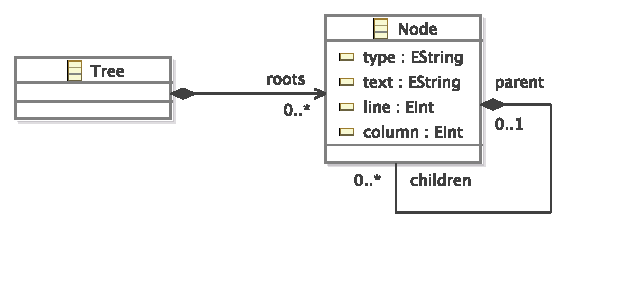
\includegraphics[width=8cm]{5.Implementation/images/ast_metamodel.pdf}
  \caption{A metamodel for abstract syntax trees, in Ecore}
  \label{fig:ast_metamodel}
\end{figure}

The abstract syntax tree produced by ANTLR can be regarded as a model (conforming to the metamodel in Figure~\ref{fig:ast_metamodel}) and hence, producing an EMF model from the abstract syntax tree can be regarded as a model-to-model transformation. Epsilon HUTN, however, was designed as two separate model-to-model transformations, for two reasons. Firstly, initial prototyping highlighted that the difference between a model represented in terms of the tree metamodel in Figure~\ref{fig:ast_metamodel} and the same model represented in metamodel-specific terms is vast, and the logic required to perform a one-step transformation quickly became complicated even for simple models. In particular, each transformation rule would have required a lengthly guard statement, which would have been difficult to debug and maintain. Secondly, it became apparent that the concrete syntax defined in OMG HUTN could be transformed to the metamodel-independent syntax defined in Section~\ref{sec:mmi_syntax}, which would reduce implementation effort by re-using the metamodel and conformance checking service described in Section~\ref{sec:mmi_syntax}.

\subsubsection{Implementation of Epsilon HUTN}
For the reasons outlined above, Epsilon HUTN is implemented using two model-to-model transformations. Figure \ref{fig:architecture} outlines the workflow through Epsilon HUTN, from HUTN source text to an EMF instantiation of the target model. The HUTN model specification is parsed to an abstract syntax tree using a HUTN parser specified in ANTLR \cite{parr07antlr}. From this, a Java postprocessor is used to construct an instance of the simple AST metamodel in Figure~\ref{fig:ast_metamodel}. Using ETL, a M2M transformation is applied to produce an intermediate model, which is an instance of the metamodel-independent syntax discussed in Section~\ref{sec:mmi_syntax}. Validation is performed on the intermediate model to ensure that the syntactic constraints specified in the OMG HUTN specification are satisfied\footnote{For example, no two objects may have the same identifier.}, and that the model conforms to the target metamodel. Conformance checking is achieved by re-using the service presented in Section~\ref{sec:mmi_syntax}. Finally, a M2T transformation on the target metamodel, specified in EGL, produces a further M2M transformation, which consumes the intermediate model and produces the target model\footnote{This final step involves a higher-order transformation (a M2T transformation is used to produce a M2M transformation), and is described in more detail below.}.

\begin{figure}[htbp]
  \begin{center}
    \leavevmode
    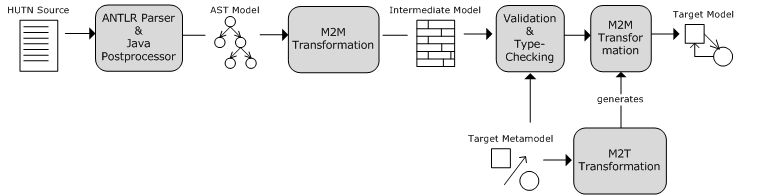
\includegraphics[scale=0.44]{5.Implementation/hutn_workflow.png}
  \end{center}
  \caption{The architecture of Epsilon HUTN.}
  \label{fig:architecture}
\end{figure}

The modular architecture in Figure~\ref{fig:architecture} facilitated the re-use of the me\-ta\-mo\-del-inde\-pe\-nd\-ent syntax and conformance checking service described in Section~\ref{sec:mmi_syntax}, and hence reduced implementation effort. A small modification was made to the metamodel-independent syntax to facilitate the implementation of Epsilon HUTN: an additional metaclass, \texttt{Pa\-ck\-a\-geOb\-je\-ct}, was added to the metamodel-independent syntax. In OMG HUTN, packages are used to segregate a model such that different parts of a OMG HUTN document can refer to different metamodels. Consequently, a \texttt{Pa\-ck\-a\-geOb\-je\-ct} has a type (i.e. the metamodel to which its contents refer), an optional identifier (used for inter-package references) and contains any number of \texttt{Ob\-je\-ct}s. To avoid confusion with \texttt{Pa\-ck\-a\-geOb\-je\-ct}, the \texttt{Ob\-je\-ct} class in the metamodel-independent syntax was renamed to \texttt{Cl\-a\-ssOb\-je\-ct}. The version of the me\-ta\-mo\-del-inde\-pe\-nd\-ent syntax used with Epsilon HUTN is shown in Figure~\ref{fig:mmi_syntax_hutn}.

\begin{figure}[htbp]
  \centering
  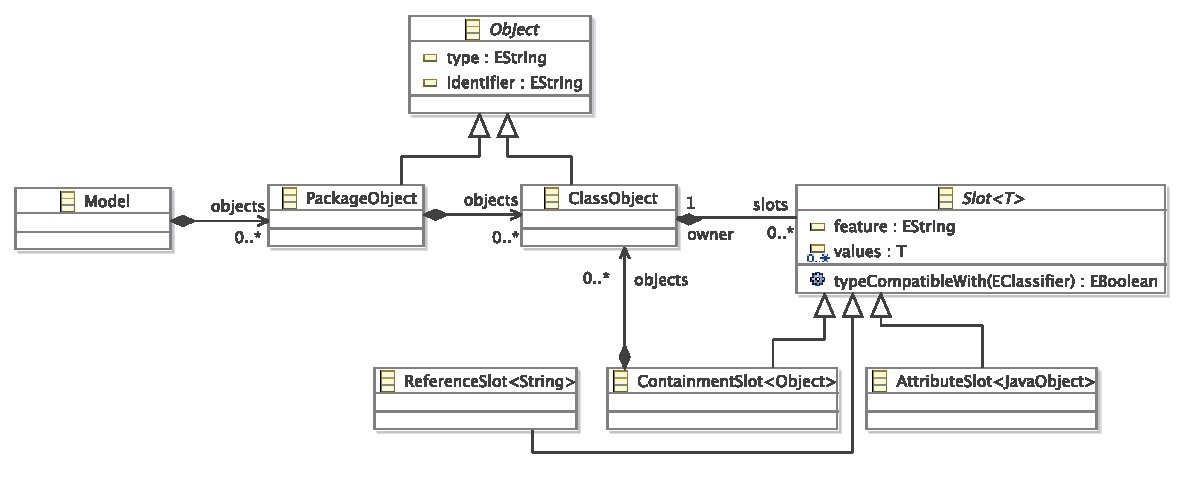
\includegraphics[width=12cm]{5.Implementation/images/slot_model_final.pdf}
  \caption{Final version of the metamodel-independent syntax, in Ecore}
  \label{fig:mmi_syntax_hutn}
\end{figure}

Each module of the architecture in Figure~\ref{fig:architecture} is now discussed in detail. Note that, in this section, instances of the metamodel-independent syntax producing during the execution of the HUTN workflow are termed an \textit{intermediate model}.

\paragraph{Parsing the HUTN Source}
A parser for OMG HUTN was constructed using ANTLR \cite{parr07antlr}, a parser generator tool. ANTLR produces a parser from an annotated EBNF grammar definition. Part of the grammar definition used by Epsilon HUTN is shown in Listing~\ref{lst:hutn_grammar} and is used to generate parser rules that process the body of \texttt{Cl\-a\-ssOb\-je\-ct}s. The \texttt{attr} rule on line 4, for example, matches any number of comma separated attribute values or the \texttt{null} keyword.

Epsilon HUTN uses a simple, bespoke Java post-processor to construct instances of the abstract syntax tree metamodel (Figure~\ref{fig:ast_metamodel}) from the Java objects produced by ANTLR. Specifically, the post-processor copies the Java objects produced by the parser into an EMF resource, and hence produces a model that can be managed with EMF.

\begin{lstlisting}[caption=An extract of the Epsilon HUTN grammar definition in EBNF, label=lst:hutn_grammar, language=EBNF]
cls_contents = feature | adjective
feature = NAME ASSIGNMENT feature_contents
feature_contents = attr | refs | containments
attr = attr_value { COMMA attr_value } | NULL
\end{lstlisting}

\paragraph{AST Model to Intermediate Model}
For M2M transformation, Epsilon HUTN uses ETL \cite{kolovos08etl}. One of the transformation rules from Epsilon HUTN is shown in Listing \ref{lst:m2m}; the complete transformation is presented in Listing~\ref{lst:m2m_full}. In Listing~\ref{lst:m2m}, the rule (starting on line 1) transforms a \texttt{No\-de} with type \texttt{na\-me} (which could represent a \texttt{P\-ac\-ka\-geOb\-je\-ct} or a \texttt{Cl\-a\-ssOb\-je\-ct}) to a \texttt{P\-ac\-ka\-geOb\-je\-ct} in the intermediate model. The guard (line 5) specifies that a name node will only be transformed to a \texttt{P\-ac\-ka\-geOb\-je\-ct} if the node has no parent (i.e. it is a top-level node, and hence a package rather than a class). The body of the rule states that the type, line number and column number of the package are determined from the text, line and column attributes of the \texttt{No\-de} object. On line 11, a \texttt{Co\-nt\-ai\-nm\-e\-ntSl\-ot} is instantiated to hold the children of this \texttt{P\-ac\-ka\-geOb\-je\-ct}. The children of the \texttt{No\-de} object are transformed to the intermediate model (using a method built into ETL, \texttt{eq\-ui\-va\-lent()}), and added to the \texttt{Co\-nt\-ai\-nm\-e\-ntSl\-ot}.

\begin{lstlisting}[caption=Transforming Nodes to PackageObjects with ETL., label=lst:m2m, language=ETL]
rule NameNode2PackageObject
    transform n : AntlrAst!Node
    to p : Intermediate!PackageObject {

    guard : n.type == 'Name' and n.parent.isUndefined()

    p.type := n.text;
    p.line := n.line;
    p.col  := n.column;

    var slot := new Intermediate!ContainmentSlot;
    for (child in n.children) {
        slot.objects.add(child.equivalent());
    }
    if (slot.objects.notEmpty()) {
        p.slots.add(slot);
    }
}
\end{lstlisting}

\paragraph{Intermediate Model Validation}
An advantage of the two-stage transformation is that contextual analysis can be specified in an abstract manner -- that is, without having to express the traversal of the AST. This gives clarity and minimises the amount of code required to define syntactic constraints.

\begin{lstlisting}[caption=A constraint (in EVL) to check that all identifiers are unique., label=lst:constraint, language=EVL]
context ClassObject {
    constraint IdentifiersMustBeUnique {
        guard: self.id.isDefined()
        check: ClassObject.all
                   .select(c|c.id = self.id).size() = 1;
        message: `Duplicate identifier: ' + self.id
    }
}
\end{lstlisting}

Epsilon HUTN uses EVL \cite{kolovos08evl} to specify validation, resulting in highly expressive syntactic constraints. An EVL constraint comprises a guard, the logic that specifies the constraint, and a message to be displayed if the constraint is not met. For example, Listing \ref{lst:constraint} specifies the constraint that every HUTN class object has a unique identifier. The complete set of constraints is presented in Listing~\ref{lst:constraints_full}.

In addition to the syntactic constraints defined in the OMG HUTN specification, the EVL constraints for checking conformance (Section~\ref{sec:mmi_syntax}) are also executed on the model at this stage.

\paragraph{Intermediate Model to Target Model}
When the intermediate model conforms to the target metamodel, the intermediate model can be transformed to an instance of the target metamodel. In other words, the model can be represented in a metamodel-specific manner and, for example, saved to disk using XMI. In generating the target model from the intermediate model (Figure \ref{fig:architecture}), the transformation uses information from the target metamodel, such as the names of classes and features. A typical approach to this category of problem is to use a higher-order transformation (HOT) on the target metamodel to generate the desired transformation \cite{tisi09hot}. Currently, ETL cannot be used to produce a transformation from a transformation and hence Epsilon HUTN uses a slightly different approach: the transformation to the target model is produced by executing a M2T transformation on the target metamodel, using EGL \cite{rose08egl}. EGL is a template-based M2T language; \verb|[% %]| tag pairs are used to denote dynamic sections, which may produce text when executed; any code not enclosed in a \verb|[% %]| tag pair is included verbatim in the generated text.

Listing \ref{lst:generate} shows part of the M2T transformation used by Epsilon HUTN; the complete M2T transformation is presented in Listing~\ref{lst:generate_full}. When executed on the target metamodel, the M2T transformation generates an ETL program (i.e. a M2M transformation). The generated ETL code transforms an intermediate model to a model that conforms to the target metamodel. The loop beginning on line 1 of Listing~\ref{lst:generate} iterates over each metaclass in the target metamodel, producing a M2M transformation rule. The generated transformation rule consumes a \texttt{Cl\-a\-ssOb\-je\-ct} in the intermediate model and produces an element of the target model. The guard of the generated transformation rule (line 6) ensures that only \texttt{Cl\-a\-ssOb\-je\-ct} with a type equal to the current meta-class are transformed by the generated rule. To generate the body of the rule, the M2T transformation iterates over each structural feature of the current meta-class, and generates appropriate transformation code for populating the values of each structural feature from the slots on the class object in the intermediate model. The part of the M2T transformation that generates the body of M2M transformation rule is omitted in Listing~\ref{lst:generate} because it contains a large amount of code for interacting with EMF, which is not relevant to this discussion. The complete M2T transformation is presented in Listing~\ref{lst:generate_full}.

\begin{lstlisting}[caption={[Higher-order transformation with EGL]Part of the M2T transformation (in EGL) that takes a target metamodel and generates an intermediate model to target model transformation (in ETL).}, label=lst:generate, language=EGL]
[% for (class in EClass.allInstances()) { %]
rule Object2[%=class.name%]
  transform o : Intermediate!ClassObject
  to t : Model![%=class.name%] {

    guard: o.type = `[%=class.name%]'

    -- body omitted
  }
[% } %]
\end{lstlisting}

To illustrate the way in which Epsilon HUTN generates a target model from an intermediate model, the M2T transformation in Listing~\ref{lst:generate} is applied to the the families metamodel in Figure~\ref{fig:original_families_mm_repeated}. The M2T transformation generates the two M2M transformation rules in Listing~\ref{lst:hutn_generated_transformation}. The rules produce instances of \texttt{Fa\-mi\-ly} and \texttt{Pe\-rs\-on} from instances of \texttt{Cl\-a\-ssOb\-je\-ct} in the intermediate model. The body of each rule copies the values from the slots of the \texttt{Cl\-as\-sOb\-je\-ct} to the \texttt{Fa\-mi\-ly} or \texttt{Pe\-rs\-on} in the target model. Lines 7-9, for example, copy the value of the name \texttt{Sl\-ot} (if one is specified) to the target \texttt{Fa\-mi\-ly}.

\begin{lstlisting}[caption=The M2M transformation generated for the Families metamodel, label=lst:hutn_generated_transformation, language=ETL, float=tb]
rule Object2Family
  transform o : Intermediate!ClassObject
  to t : Model!Family {

    guard: o.type = 'Family'

    if (o.hasSlot('name')) {
			t.name := o.findSlot('name').values.first;
		}
		
		if (o.hasSlot('address')) {
			for (value in o.findSlot('address').values) {
				t.address.add(value);
			}
		}
		
		-- remainder of body omitted
  }

rule Object2Person
  transform o : Intermediate!ClassObject
  to t : Model!Person {

    guard: o.type = 'Person'

    if (o.hasSlot('name')) {
			t.name := o.findSlot('name').values.first;
		}
		
		-- remainder of body omitted
  }
\end{lstlisting}

Currently, Epsilon HUTN can be used only to generate EMF models. Support for other modelling languages would require different transformations between intermediate and target model. In other words, for each target modelling language, a new EGL template would be required. The transformation from AST to intermediate model is independent of the target modelling language and would not need to change. As EMF is arguably the most widely-used modelling framework today, support for other modelling frameworks is not crucial for exploring the suitability of HUTN for user-driven co-evolution. However, one interesting example of metamodel evolution predates EMF: the changes made to UML between versions 1.5 and 2.0 of the specification. Because the UML 1 specifications use a version of MOF that is not supported by EMF, the current version of Epsilon HUTN cannot be used for migrating UML 1 models. Several other examples, however, were available for evaluating Epsilon HUTN, and so support for other modelling frameworks was not crucial in the context of the thesis research.

\subsubsection{Compliance to OMG HUTN}
Epsilon HUTN is a reference implementation of the OMG HUTN standard. There are, however, a few differences between the implementation in Epsilon and the OMG standard. The differences are now discussed and justified. The discussion is based on\footnote{\url{http://www.eclipse.org/gmt/epsilon/doc/articles/hutn-compliance/}}, which provides an up-to-date report of Epsilon HUTN's compliance to the OMG HUTN standard.

\begin{table}
	\centering
	\begin{tabular}{|c|c|c|}
		\hline
		\textbf{OMG HUTN} & \multicolumn{2}{|c|}{\textbf{Epsilon HUTN}} \\
		\hline
		\textbf{Feature} & \textbf{Supported?}          & \textbf{Details of support} \\
		\hline
		\hline
		Packages                                    & Yes                       & \\
		\hline                                                                    
		\multirow{3}{*}{Classes}                    & \multirow{3}{*}{Partial}  & Not yet supported:      \\
		                                            &                           & parametric attributes,  \\
		                                            &                           & enumeration adjectives. \\
		\hline                                                                    
		\multirow{2}{*}{Attributes}                 & \multirow{2}{*}{Yes}      & Corrects a mistake \\
		                                            &                           & in the standard. \\
		\hline                                                                    
		References                                  & Yes                       & \\
		\hline                                                                                   
		Classifier-level attributes                 & Yes                       & \\
		\hline                                                                                   
		Data values                                 & Yes                       & \\
		\hline                                                     
		\multirow{2}{*}{Inline configuration (6.9)} & \multirow{2}{*}{No}       & A configuration model \\
		                                            &                           & is used instead. \\
		\hline
		\multirow{3}{*}{Configuration rules (5)}    & \multirow{3}{*}{Partial}  & Not yet supported:      \\
		                                            &                           & parametric attributes,  \\
		                                            &                           & enumeration adjectives. \\
		\hline
	\end{tabular}
	\label{tab:hutn}
	\caption{Compliance of Epsilon HUTN to OMG HUTN}
\end{table}

Table~\ref{tab:hutn} summarises the differences between Epsilon HUTN and the OMG HUTN standard. Epsilon HUTN does not support two of the syntactic shortcuts described for classes in the OMG HUTN standard: parametric attributes and enumeration adjectives. The former are used to specify attribute values in a parametric form (e.g. \texttt{Point (0,0)}, for creating a \texttt{Po\-i\-nt} object with \texttt{x} and \texttt{y} attributes with value 0). The latter allows an enumeration value to prefix an object definition (e.g. \texttt{female Person} for creating a \texttt{Pe\-rs\-on} with \texttt{fe\-ma\-le} gender). The attribute to which the parametric or enumeration values are bound is specified using OMG HUTN configuration rules (Section~\ref{subsec:hutn}). Parametric attribute and enumeration adjectives were not implemented to reduce the amount of time required to build Epsilon HUTN. Alternative (albeit less concise) notion can be used to express models without using parametric attribute and enumeration adjectives.

Section 6.4 of the OMG HUTN standard \cite{hutn} appears to contain a mistake in the grammar definition. Grammar rule 20 implies that an attribute's name is optional when specifying a keyword attribute, and that an empty string or a tilde character are valid forms of a keyword attribute. However, the prose describing grammar rule 20 proposes no semantics for an empty string or a tilde character as a keyword attribute. Consequently, Epsilon HUTN deviates from grammar rule 20 of the OMG HUTN standard, and requires an attribute name for every keyword attribute.

Finally, the OMG HUTN standard defines syntax for specifying configuration rules \emph{inline}, at the start of a HUTN document. Epsilon HUTN does not support inline configuration, and Epsilon HUTN documents are configured with a configuration model, which is constructed using an EMF model editor. Using a configuration model rather than inline configuration reduced the time required to implement Epsilon HUTN and facilitated re-use of configuration models between HUTN documents.

The OMG HUTN standard does not include a set of compliance tests for reference implementations. Instead, the compliance of Epsilon HUTN to OMG HUTN was checked using the many examples of HUTN documents in the OMG HUTN standard \cite{hutn}. The examples were used to create a suite of executable compliance test cases, which were run frequently during the development of Epsilon HUTN.
 

\subsection{Migration with Epsilon HUTN}
\label{subsec:migration_with_hutn}
Used in combination with the metamodel-independent syntax presented in Section~\ref{sec:mmi_syntax}, Epsilon HUTN facilitates user-driven co-evolution using the workflow in Section~\ref{fig:hutn_process_implementation}, which provides an alternative to the user-driven co-evolution workflow observed in Section~\ref{subsec:user-driven_co-evolution}. First, the user attempts to load a model in the model editor\footnote{The workflow in Figure~\ref{fig:hutn_process_implementation} assumes a graphical model editor, such as those generated by GMF, but any editor built atop EMF will exhibit the same behaviour.}. If the model is non-conformant and cannot be loaded, the user clicks a ``Generate HUTN'' menu item provided by Epsilon HUTN. Epsilon HUTN then binds the model to the metamodel-independent syntax and unparses the bound model to produce HUTN source code equivalent to XMI representation of the non-conformant model.

To support the final step of the workflow in Figure~\ref{fig:hutn_process_implementation}, Epsilon HUTN provides an editor for HUTN documents that is integrated with the conformance checking service described in Section~\ref{sec:mmi_syntax}. The user edits the HUTN document to reconcile conformance problems (i.e. perform migration), and Epsilon HUTN automatically performs conformance checking as the user edits the HUTN document. When the conformance problems are fixed, the user saves the HUTN document and Epsilon HUTN automatically generates XMI for the conformant model (using the model transformations described in Section~\ref{subsec:epsilon_hutn}). The conformant model can then be loaded in the model editor.

\begin{figure}[htbp]
	\centering
	\includegraphics*[viewport=80 290 760 550,height=4.75cm]{6.Evaluation/images/user_driven/hutn_process.pdf}
	\caption{User-driven co-evolution with dedicated structures}
	\label{fig:hutn_process_implementation}
\end{figure}

To demonstrate the way in which HUTN can be used to perform migration, the XMI shown in Listing~\ref{lst:xmi} is represented using OMG HUTN in Listing~\ref{lst:non-conformant_hutn}. Recall that the XMI describes a \texttt{Fa\-mi\-ly} with one adopted and one natural child.

\begin{lstlisting}[caption=OMG HUTN for people with mothers and fathers., label=lst:non-conformant_hutn, language=HutnFamilies]
FamilyPackage "families" {
    Family "Smiths" {
	      name: "Smiths"
	      naturalChildren: Person { name: "Paul" }
		    adoptedChildren: Person { name: "John" }
		}
}
\end{lstlisting}

If the Families metamodel now evolves such that children are modelled using one rather than two features (Figure~\ref{fig:evolved_families_mm_repeated}), Epsilon HUTN reports conformance problems on the HUTN document using the conformance checking service described in Section~\ref{sec:mmi_syntax}, as illustrated by the screenshot in Figure~\ref{fig:hutn_conformance_reporting}.

\begin{figure}[htbp]
  \begin{center}
    \leavevmode
    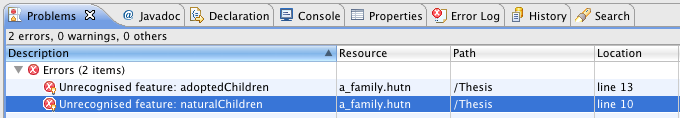
\includegraphics[scale=0.44]{5.Implementation/hutn_conformance_reporting.png}
  \end{center}
  \caption{Conformance problem reporting in Epsilon HUTN.}
  \label{fig:hutn_conformance_reporting}
\end{figure}

Resolving the conformance problems requires the user to merge the values for \texttt{ad\-op\-t\-edCh\-il\-dr\-en} and \texttt{na\-tu\-ralCh\-il\-dr\-en} into a set of values for the new feature, \texttt{ch\-il\-dr\-en}. The Epsilon HUTN development tools provide content assistance, which might be useful in this situation. Listing~\ref{lst:conformant_hutn} shows a HUTN document that conforms to the evolved metamodel in which adopted and natural children are specified using a single feature, \texttt{ch\-il\-dr\-en}.

\begin{lstlisting}[caption=HUTN for people with parents., label=lst:conformant_hutn, language=HutnFamilies]
FamilyPackage "families" {
    Family "Smiths" {
	      name: "Smiths"
	      children: Person { name: "Paul" },
                  Person { name: "John" }
		}
}
\end{lstlisting}

When the user saves the reconciled HUTN document, Epsilon HUTN will automatically generate XMI for the (now) conformant model, and migration is complete. Compared to the user-driven co-evolution workflow observed in Section~\ref{subsec:user-driven_co-evolution}, the workflow presented in Figure~\ref{fig:hutn_process_implementation} provides live conformance checking and a modelling notation that is optimised for humans rather than for machines. The two workflows are compared and evaluated in Chapter~\ref{Evaluation}.

\subsection{Summary}
In this section, a textual modelling notation for performing model migration has been designed and implemented. The notation proposed in this section is based on the OMG HUTN standard, which was described in Section~\ref{subsec:hutn}. The design and implementation of Epsilon HUTN, an implementation of OMG HUTN for EMF, was discussed in this section. Integration of Epsilon HUTN with the metamodel-independent syntax in Section~\ref{sec:mmi_syntax} facilitates user-driven co-evolution with a textual modelling notation other than XMI, as demonstrated by the example above. The user-driven co-evolution workflow presented in Section~\ref{subsec:migration_with_hutn} is evaluated in Chapter~\ref{Evaluation}. The remainder of this chapter focuses on developer-driven co-evolution, in which model migration strategies are executable.